\chapter{Overall Description}

\section{Product perspective}

The system will be developed from scratch and it will completely replace the legacy system. \newline
It is composed by a client part and a server part.
The latter is composed by an application server (CLup Server) where all the logic is located. It also comprehends the web server, the database server and the mail server,
which all communicate with the CLup Server.
It has an interface, the API Manager, which exposes the public CLup API, for the QR validation. It also makes use of an External Map API for querying data about the 
distance of the user from the store. This information will be used to inform the user of when leave the current place.\newline
The solution for the client part includes two interfaces based on the user type: the mobile app for the customers and the browser for supermarkets' employee and managers.
\begin{figure}[H]
	\centering
	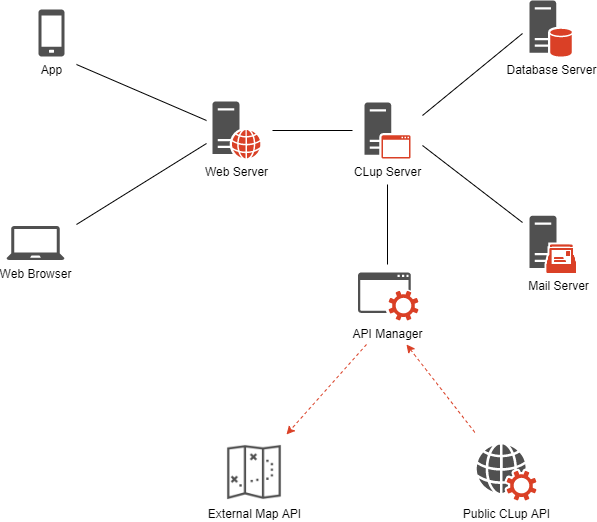
\includegraphics[scale=0.45]{ProdPerspective_Diagram}
	\caption{CLup system diagram}	
\end{figure}	 

\section{Product functions}
This section provides a summary of the major functions that the software will perform w.r.t. the goals already described in section <<SECTION>> \todo{Add right section}.

\subsection{Queue function}
The main function of \textit{CLup} is to manage queues. A user who wants to do grocery-shopping will join the queue for a specific store through the Mobile App.\newline
Firstly, the user will be asked to select the store in which he desires to line-up.\newline
Then the system will prompt the current size of the queue and an estimate of waiting time. If the user is satisfied with his choice it can subscribe to the queue, operation that will be confirmed by the emission of a ticket. The ticket comprehends a queue number, which identify user's position in the queue, and a QR code, which is used for the ticket validation. At any time the user will be able to check his position in the and the \textit{leave-at-time} (i.e. the time they need to depart from their current position to reach the store); the current position will be retrieved by the GPS of the user device. This requires the GPS service to be enabled, otherwise no time estimation will be shown.

\subsection{Reserve function}
This advanced function allows customers to "book a visit" to the store. Customers are asked to select the store they want to visit. Then they need to fill in a form by indicating:
\begin{itemize}
	\item an \textbf{email address}, which will be needed to send a receipt and memo to the user;
	\item the \textbf{date} and \textbf{time} of the visit;
	\item the approximate \textbf{expected duration} of the trip;
 	\item the main \textbf{categories of items} they intend to buy.
\end{itemize}
Every field of the form is mandatory, this means that the user must complete all of them in order to submit the reservation. %The more specific is the user the more effective is \textit{CLup}.

In addition, for long-term customers, it also suggests a time inferred by the system based on an analysis of the previous visits.
Customers are also allowed to delete their booking at any time by going to the right section in the Mobile App or by clicking the link sent via email after the reservation. 

\subsection{Validation function}
The system provides an API interface that can be queried to allow the validation of QR codes. The process of scanning the QR is to be handled by an external service.
% Add what we need QR for and why we validate them. (Fake tickets)
\todo{Check comments}

\subsection{Dashboard function}
\textit{Customers Line-up} web platform grants supermarkets a way to manage queues and customers inside their stores. In particular, it offers two level of access: \textit{manager-level} and \textit{staff-level}.

\begin{itemize}
	\item \textbf{Manager-level}\newline
	With the \textbf{dashboard UI}, store managers have access to tables and data visualizations of their customers visits and behaviours. In particular, they can monitor the number of people in the queue and the ones inside the store. Then, based on those data they can setup the maximum cap of people in the store and in the queue.\newline
	Store managers can view, edit and delete the list of reservations made by the customer.\newline
	Last but not least, they can inspect statistics about the customers flow and the journey map of all the clients inside the store at any given time.

	\item \textbf{Staff-level}\newline
	A store employee is able to view data about the number of people in the queue and inside the building. This is needed during the validation of tickets when the check-in staff scans QR and allows customers inside the store.
\end{itemize}

\section{User characteristics}

\section{Constraints}

\section{Assumptions and Dependencies}

\subsection{Domain assumptions}
